\section{Normalizing Flows}
\label{section:probmodel}

\subsection{Introduction}
The best-known and most studied probability distributions, which are analitically
manageable, are rarely expressive enough for real-world complex datasets, such
as images or signals. However, they have properties that make them amenable to
work with, for instance, they allow for tractable parameter estimation,
they have closed-form likelihood functions, and sampling from them is simple.

One way to obtain more expressive models is to assume the existence of latent variables, leverage certain factorization
structures, and use well-known distributions for the individual factors of the product that
constitutes the model's joint distribution. By using these structures and
specific, well-chosen combinations of distributions (namely, conjugate prior-likelihood pairs),
these models are able to remain tractable - normally via bespoke estimation/inference/learning
algorithms.

Another approach to obtaining expressive probabilistic models is to apply
transformations to a simple distribution, and use the \emph{change of variables}
formula to compute probabilities in the transformed space. This is the basis
of \emph{normalizing flows}, an approach proposed by \textcite{shakir_nf},
and which has since evolved and developed into the basis of multiple state-of-the-art
techniques for density modelling and estimation \autocite{Glow}, \autocite{real-nvp}, \autocite{bnaf19},
\autocite{maf}.

\subsection{Change of Variables}
\label{cov}
Given a random variable $\bm{z} \in \mathbb{R}^D$, with probability density function $f_Z$,
and a bijective and continuous function $g(\: . \: ;\bm\theta)\ : \ \mathbb{R}^D\rightarrow \mathbb{R}^D$,
the probability density function $f_X$ of the random variable $\bm{x} = g(\bm{z})$ is given by
\begin{align}
    f_X(\bm{x}) &= f_Z(g^{-1}(\bm{x};\bm\theta))\Big|\det\Big(\frac{d}{d\bm{x}}g^{-1}(\bm{x};\bm\theta)\Big)\Big| \\
    &= f_Z(g^{-1}(\bm{x};\bm\theta))\Big|\det\Big(\frac{d}{d\bm{z}}g(\bm{z};\bm\theta) \bigg{|}_{\bm{z} = g^{-1}(\bm{x};\bm\theta)}\Big)\Big|^{-1},
\end{align} where $\det\Big(\frac{d}{d\bm{x}}g^{-1}(\bm{x};\bm\theta)\Big)$
is the determinant of the Jacobian matrix of $g^{-1}(\: . \: ;\bm\theta)$,
computed at $\bm{x}$.
Since $g(\: . \: ;\bm\theta)$ is a transformation parameterized by a parameter
vector $\bm\theta$, this expression can be optimized w.r.t. $\bm\theta$, with the
goal of making it approximate some arbitrary distribution. For this to be feasible,
the following have to be easily computable:
\begin{itemize}
    \item $f_Z$ - the starting probability density function
        (also called \emph{base density}). It is assumed that it has a closed-form
        expression. In practice, this is typically one of the basic distributions
        (Gaussian, Uniform, etc.)
    \item $\det\Big(\frac{d}{d\bm{x}}g^{-1}(\bm{x};\bm\theta)\Big)$ - the determinant
        of the Jacobian matrix of $g^{-1}$; for most transformations, this is not
        \q{cheap} to compute.
    \item The gradient of $\det\Big(\frac{d}{d\bm{x}}g^{-1}(\bm{x};\bm\theta)\Big)$
        w.r.t. $\bm\theta$; this is crucial for gradient-based optimization of
        $\bm\theta$ to be feasible. For most cases, this is not easily computable.
\end{itemize}
As will become clear, the crux of the \emph{normalizing flows} framework is to find
transformations that are expressive enough, and for which the determinants of their
Jacobian matrices, as well as the gradients of those determinants are both \q{cheap}
to compute.

\subsection{Normalizing Flows}
Consider $L$ transformations $h_\ell$, for $\ell = 0, 1, ..., L-1$ that fulfill the
three requirements listed above. Let each of those transformations be parameterizable
by a parameter vector $\bm\theta_\ell$, for $\ell = 0, 1, ..., L-1$. The
dependence on the parameter vectors will be implicit from here on.
Let $\bm{z_\ell} = h_{\ell-1} \circ h_{\ell-2} \circ ... \circ h_0(\bm{z_0})$, where
$\bm{z_0}$ is sampled from $f_Z$, the base density. Notice that, with this notation,
$\bm{z_L} = \bm{x}$. Furthermore, let $g$ be the composition of the $L$ transformations.
Applying the change of variables formula to
\begin{align}
    \bm{z_0} &\sim f_Z \\
    \bm{x} &= h_{L-1} \circ h_{L-2} \circ ... \circ h_0(\bm{z_0}),
\end{align}
noting that $g^{-1} = h^{-1}_0 \circ h^{-1}_1 \circ ... \circ h^{-1}_{L-1}$ and
using the chain rule for derivatives, leads to
\begin{align}
    f_X(\bm{x}) &= f_Z(g^{-1}(\bm{x}))\Big|\det\Big(\frac{d}{d\bm{x}}g^{-1}(\bm{x})\Big)\Big| \\
                        &= f_Z(g^{-1}(\bm{x}))\prod_{\ell=0}^{L-1}\Big|\det\Big(\frac{d}{d\bm{z_{\ell+1}}}h_{\ell}^{-1}(\bm{z_{\ell+1}})\Big)\Big| \\
                        &= f_Z(g^{-1}(\bm{x}))\prod_{\ell=0}^{L-1}\Big|\det\Big(\frac{d}{d\bm{x_{\ell}}}h_{\ell}(\bm{x_\ell})\bigg{|}_{\bm{x_\ell} = h_{\ell}^{-1}(\bm{z_{\ell+1}})}   \Big)\Big|^{-1} \label{eq:nflowderivation}
\end{align}
Replacing $h_{\ell}^{-1}(\bm{z_{\ell+1}}) = \bm{z_\ell}$ in (\ref{eq:nflowderivation}) leads to
\begin{align}
         f_X(\bm{x}) = f_Z(g^{-1}(\bm{x}))\prod_{\ell=0}^{L-1}\Big|\det\Big(\frac{d}{d\bm{z_{\ell}}}h_{\ell}(\bm{z_\ell})\Big)\Big|^{-1};
\end{align} taking the logarithm,
\begin{align}
    \log f_X(\bm{x}) = \log f_Z(g^{-1}(\bm{x})) - \sum_{\ell=0}^{L-1} \log \Big|\det\Big(\frac{d}{d\bm{z_{\ell}}}h_{\ell}(\bm{z_\ell})\Big) \Big|. \label{eq:nflowsfinal}
\end{align}
Depending on the task, one might prefer to replace the second term in (\ref{eq:nflowsfinal})
with a sum of log-absolute-determinants of the Jacobians of the inverse transformations.
This choice would imply replacing the minus sign before the sum with a plus sign:
\begin{align}
    &\log f_X(\bm{x}) = \nonumber \\
    &= \log f_Z(g^{-1}(\bm{x})) + \sum_{\ell=0}^{L-1} \log \Big|\det\Big(\frac{d}{d\bm{z_{\ell+1}}}h_{\ell}^{-1}(\bm{z_{\ell+1}})\Big) \Big|.
\end{align}
We started by assuming that the transformations $h_\ell$ fulfill the requirements
listed in Section \ref{cov}. For that reason, it is clear that the above expression
is a feasible objective for gradient-based optimization. In practice, this is carried
out by leveraging modern automatic differentiation and optimization frameworks \autocites{flowpp, Glow, real-nvp}.
Sampling from the resulting distribution is simply achieved by sampling from the base
distribution and applying the chain of transformations. Because of this, normalizing
flows can be used as flexible variational posteriors, in variational
inference settings, as well as density estimators.

\subsection{Examples of transformations}
\subsubsection{Affine Transformation}
An affine transformation is arguably the simplest choice; it can
stretch, sheer, shrink, rotate, and translate the space. It is simply achieved
by the multiplication by a matrix $A$ and summation of a bias vector $\bm{b}$:
\begin{align}
    \bm{z} &\sim p(\bm{z}) \\
    \bm{x} &= A\bm{z} + \bm{b}.
\end{align}
The determinant of the Jacobian of this transformation is simply the determinant
of $A$. However, in general, computing the determinant of a $D \times D$
matrix has $\mathcal{O}(D^3)$ computational complexity. For that reason, it is
common to use matrices with a certain structure that makes their determinants
easier to compute. For instance, if $A$ is triangular, its determinant is
the product of its diagonal's elements. The downside of using matrices that are
constrained to a certain structure is that they correspond to less flexible transformations.

It is possible, however, to design affine transformations whose Jacobian determinants
are of $\mathcal{O}(D)$ complexity and that are more expressive than simple
triangular matrices. \textcite{Glow} propose one such transformation. It
constrains the matrix $A$ to be decomposable as ${A = PL\big(U + \mbox{diag}(\bm{s})\big)}$,
where $\mbox{diag}(\bm{s})$ is a diagonal matrix whose diagonal's elements are
the components of vector $\bm{s}$. The following additional constrains are in place:
\begin{itemize}
    \item $P$ is a permutation matrix
    \item $L$ is a lower triangular matrix, with ones in the diagonal
    \item $U$ is an upper triangular matrix, with zeros in the diagonal
\end{itemize}
Given these constraints, the determinant of matrix $A$ is simply the product
of the elements of $\bm{s}$.

\begin{figure}[!htb]
  \begin{subfigmatrix}{2}
    \subfigure[]{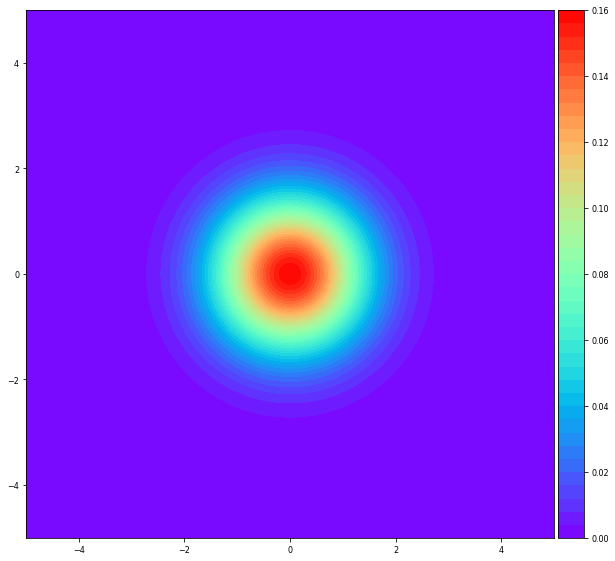
\includegraphics[width=0.49\linewidth]{figures/base_distribution.png}}
    \subfigure[]{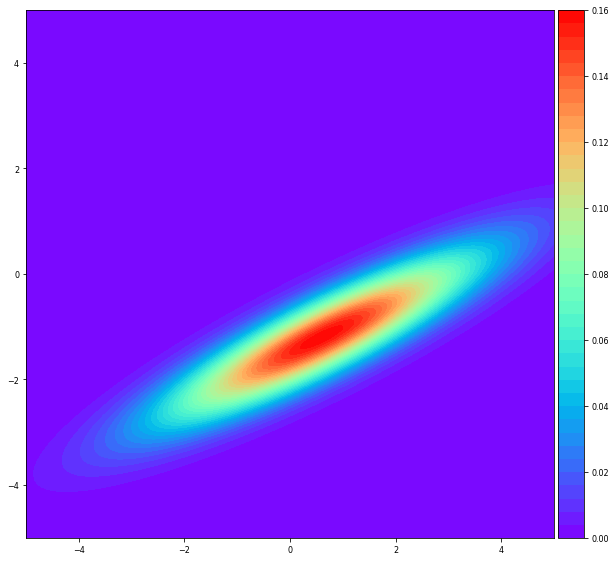
\includegraphics[width=0.49\linewidth]{figures/affine_transform.png}}
  \end{subfigmatrix}
    \caption{(a) Density of a Gaussian distribution with $\mu = [0, 0]$ and $\Sigma = I$
    (b) Density of the distribution that results from applying some affine transformation to
    the Gaussian distribution in (a)
    }
  \label{fig:affine}
\end{figure}

\subsubsection{PReLU Transformation}
Intuitively, introducing non-linearities endows normalizing flows with more flexibility to
represent complex distributions. This can be done in a similar fashion to the
activation functions used in neural networks. One example of that is the parameterized
rectified linear unit (PReLU) transformation. It is defined in the following manner, for
a $D$-dimensional input:
\begin{align}
f(\bm{z}) = [f_1(z_1), f_2(z_2), ..., f_D(z_D)],
\end{align} where
\begin{align}
f_i(z_i) =
    \begin{cases}
        z_i,              & \text{if } z_i\geq 0, \\
        \alpha z_i,       & \text{otherwise}.
    \end{cases}
\end{align}
In order for the transformation to be invertible, it is necessary
that $\alpha > 0$.
Let us define a function $j(.)$ as
\begin{align}
j(z_i) =
    \begin{cases}
       1 ,              & \text{if } z_i \geq 0, \\
       \alpha ,       & \text{otherwise};
    \end{cases}
\end{align}
it is trivial to see that the Jacobian of the transformation is a diagonal
matrix, whose diagonal elements are $j(z_i)$:
\begin{align}
  J(f(z)) =
  \begin{bmatrix}
      j(z_1) & & & \\
      & j(z_2) & & \\
      & & \ddots & \\
      & & & j(z_D)
  \end{bmatrix}.
\end{align}
With that in hand, it is easy to arrive at the log-absolute-determinant of this transformation's
Jacobian, which is given by $\sum_{i=1}^D \log \big| j(z_i) \big|$

\begin{figure}[!htb]
  \begin{subfigmatrix}{2}
    \subfigure[]{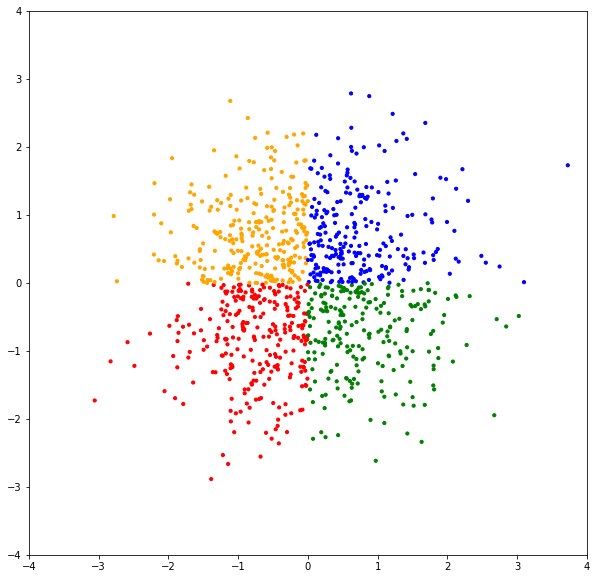
\includegraphics[width=0.49\linewidth]{figures/gaussian_in_quadrants.png}}
    \subfigure[]{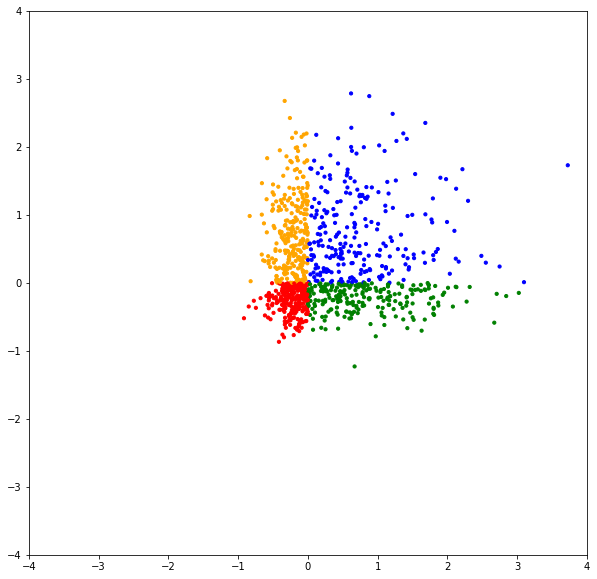
\includegraphics[width=0.49\linewidth]{figures/prelu_in_quadrants.png}}
  \end{subfigmatrix}
    \caption{(a) Samples from of a Gaussian distribution with $\mu = [0, 0]$ and $\Sigma = I$.
    The samples are colored according to the quadrant they belong to. (b) Samples from the
    distribuion in a) transformed by a PReLU transformation.}
  \label{fig:prelu}
\end{figure}

\begin{figure}[!htb]
  \begin{subfigmatrix}{3}
    \subfigure[]{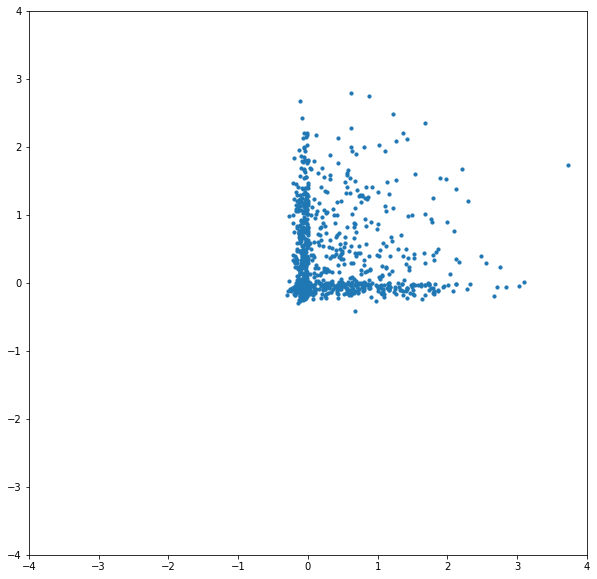
\includegraphics[width=0.31\linewidth]{figures/prelu_0_1.png}}
    \subfigure[]{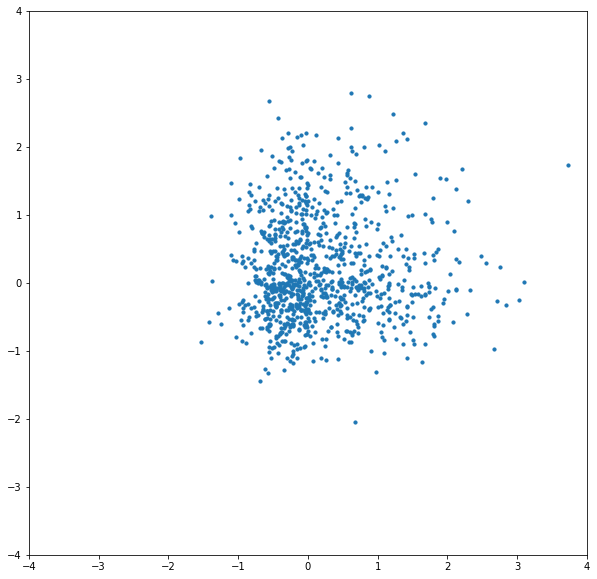
\includegraphics[width=0.31\linewidth]{figures/prelu_0_5.png}}
    \subfigure[]{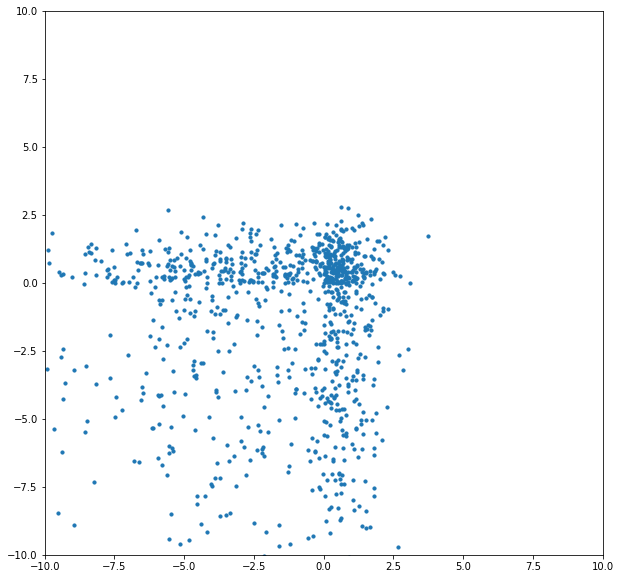
\includegraphics[width=0.31\linewidth]{figures/prelu_5.png}}
  \end{subfigmatrix}
    \caption{Samples from a Gaussian with $\mu = [0, 0]$ and $\Sigma = I$, transformed
    by PReLU transformations with different $\alpha$ parameters. (a) $\alpha = 0.1$
    (b) $\alpha = 0.5$ (c) $\alpha = 5$}
  \label{fig:prelu}
\end{figure}

\subsubsection{Batch-Normalization Transformation}
\textcite{real-nvp} propose a batch-normalization transformation, similar to
the well-known batch-normalization layer normally used in neural networks. This
transform simply applies a rescaling, given the batch mean $\tilde\mu$ and variance
${\tilde\sigma}^2$:
\begin{align}
    f(z) = \frac{z - \tilde\mu}{\sqrt{{\tilde\sigma}^2 + \epsilon}},
\end{align} where $\epsilon \ll 1$ is a term used to ensure that there never is
a division by zero. This transformation's Jacobian is trivial: 
\begin{align}
    \prod_{i=1}^D \frac{1}{\sqrt{{\tilde\sigma}_i^2 + \epsilon}}.
\end{align}

\subsubsection{Affine Coupling Transformation}
As mentioned previously, one of the active research challenges within the
normalizing flows framework is the search and design of transformations that
are sufficiently expressive and whose Jacobians are not computationally heavy. One brilliant
example of such transformations, proposed by \textcite{real-nvp}, is
called affine coupling layer.

This transformation is characterized by two arbitrary functions $s(.)$ and
$t(.)$, as well as a mask that splits an input $\bm{z}$ of dimension $D$ into
two parts, $\bm{z_1}$ and $\bm{z_2}$. In practice, $s(.)$ and $t(.)$ are neural
networks, whose parameters are to be optimized so as to make the transformation
approximate the desired output distribution. The outputs of $s(.)$ and $t(.)$
need to have the same dimension as $\bm{z_1}$. This should be taken into account when
designing the mask and the functions $s(.)$ and $t(.)$. The transformation is defined as:
\begin{align}
    \begin{cases}
    \bm{x_1} &= \bm{z_1} \odot \exp\big(s(\bm{z_2})\big) + t(\bm{z_2}) \\
    \bm{x_2} &= \bm{z_2}.
    \end{cases}
\end{align}
To see why this transformation is suitable to being used within the framework
of normalizing flows, let us derive its Jacobian.
\begin{itemize}
    \item $\frac{\partial \bm{x_2}}{\partial \bm{z_2}} = I$, because $\bm{x_2} = \bm{z_2}$.
    \item $\frac{\partial \bm{x_2}}{\partial \bm{z_1}}$ is a matrix of zeros, because $\bm{x_2}$ does not depend on $\bm{z_1}$.
    \item $\frac{\partial \bm{x_1}}{\partial \bm{z_1}}$ is a diagonal matrix,
        whose diagonal is simply given by $\exp\big(s(\bm{z_2})\big)$, since those values are
        constant w.r.t $\bm{z_1}$ and they are multiplying each element of $\bm{z_1}$.
    \item $\frac{\partial \bm{x_1}}{\partial \bm{z_2}}$ is not needed,
        as will become clear ahead.
\end{itemize}

Writing the above in matrix form:
%\[
%\begin{bmatrix}
%  \mbox{\huge$\frac{\partial \bm{x_1}}{\partial \bm{z_1}}$} & \mbox{\huge$\frac{\partial \bm{x_1}}{\partial \bm{z_2}}$} \\
%  \mbox{\huge$\frac{\partial \bm{x_2}}{\partial \bm{z_1}}$} & \mbox{\huge$\frac{\partial \bm{x_2}}{\partial \bm{z_2}}$} \\
%\end{bmatrix}
%\]


\begin{align}
    J_{f(z)} &=
        \begin{tikzpicture}[decoration=brace, baseline=-\the\dimexpr\fontdimen22\textfont2\relax ]
            \matrix (m) [matrix of math nodes,left delimiter=[,right delimiter={]}, ampersand replacement=\&] {
                \mbox{\Large$\frac{\partial \bm{x_1}}{\partial \bm{z_1}}$} \& \mbox{\Large$\frac{\partial \bm{x_1}}{\partial \bm{z_2}}$} \\
                \mbox{\Large$\frac{\partial \bm{x_2}}{\partial \bm{z_1}}$} \& \mbox{\Large$\frac{\partial \bm{x_2}}{\partial \bm{z_2}}$} \\
            };
%            \draw[decorate,transform canvas={xshift=-1.5em},thick] ($ (m-1-1.south west) +(0,3pt) $)
%                -- node[left=2pt] {$\frac{\partial \bm{x_1}}{\partial (.)}$} ($ (m-1-1.north west) -(0,3pt) $);
%            \draw[decorate,transform canvas={xshift=-1.5em},thick] ($ (m-2-1.south west) +(0,3pt) $)
%                -- node[left=2pt] {$\frac{\partial \bm{x_2}}{\partial (.)}$} ($ (m-2-1.north west) -(0,3pt) $);
%            \draw[decorate,transform canvas={yshift=0.5em},thick] ($ (m-1-1.north west) +(2pt,0) $)
%                -- node[above=2pt] {$\frac{\partial (.)}{\partial \bm{z_1}}$} ($ (m-1-1.north east) -(2pt,0) $);
%            \draw[decorate,transform canvas={yshift=0.5em},thick] ($ (m-1-2.north west) +(2pt,0) $)
%                -- node[above=2pt] {$\frac{\partial (.)}{\partial \bm{z_2}}$} ($ (m-1-2.north east) +(2pt,0) $);
        \end{tikzpicture} \\
    &=
        \begin{tikzpicture}[decoration=brace, baseline=-\the\dimexpr\fontdimen22\textfont2\relax ]
            \matrix (m) [matrix of math nodes,left delimiter=[,right delimiter={]}, ampersand replacement=\&] {
                \mbox{diag}\Big(\exp\big(s(\bm{z_2})\big)\Big) \& \mbox{\Large$\frac{\partial \bm{x_1}}{\partial \bm{z_2}}$} \\
                \mbox{\Large$\bm{0}$} \& \mbox{\Large$I$} \\
            };
        \end{tikzpicture}
\end{align} shows that the Jacobian matrix is (upper) triangular. Its determinant - the
only thing we need, in fact - is therefore easy to compute: it is simply the
product of the diagonal elements. Moreover, part of the diagonal is simply
composed of ones. The determinant, and the log-absolute-determinant become
\begin{align}
    \det\big(J_{f(z)}\big) &= \prod_i \exp\big(s(\bm{z_2}^{(i)})\big) \\
    \log \Big|\det\big(J_{f(z)}\big)\Big| &= \sum_i s(\bm{z_2}^{(i)}),
\end{align} where $\bm{z_2^{(i)}}$ is the $i$-th element of $\bm{z_2}$.
Since a single affine coupling layer does not transform all of the elements in
$\bm{z}$, in practice several layers are composed, and each layer's mask is changed
so as to make all dimensions affect each other. This can be done, for instance, with
a checkerboard pattern, which alternates for each layer. In the case of image inputs,
the masks can operate at the channel level.

\subsubsection{Masked Autoregressive Flows}
Another ingenious architecture for normalizing flows has been proposed by \textcite{maf}.
It is called masked autoregressive flow (MAF). Let $\bm{z}$ be a sample from
some base distribution, with dimension $D$. MAF transforms $\bm{z}$ into an
observation $\bm{x}$, of the same dimension, in the following manner:
\begin{align}
x_i = z_i \exp(\alpha_i) + \mu_i \\
(\mu_i, \alpha_i) = g(\bm{x_{1:i-1}}).
\end{align}
In the above expression $g$ is some arbitrary function. The inverse transform of
MAF is trivial, because, like the affine coupling layer, MAF uses $g$ to parameterize
a shift, $\mu$, and a log-scale, $\alpha$, which translates to the fact that the
function $g$ itself does not need to be inverted:
\begin{align}
z_i = (x_i - \mu_i)\exp(-\alpha_i).
\end{align}
Moreover, the autoregressive structure of the transformation constrains the
Jacobian to be triangular, which renders the determinant effortless to compute: 
\begin{align}
\det\big( J_{f(\bm{z})} \big) &= \prod_{i=1}^{D} \exp(\alpha_i), \\
\log \Big| \det \big( J_{f(\bm{z})} \big) \Big| &= \sum_{i=1}^{D} \alpha_i.
\end{align}
As stated above, the function $g$ used to obtain $\mu_i$ and $\alpha_i$ can be
arbitrary. However, in the original paper, the function proposed a masked
autoencoder for distribution estimation (MADE), as described by \textcite{MADE}.

Much like the partitioning in the affine coupling layer, the assumption of
autoregressiveness (and the ordering of the elements of $\bm{x}$
for which that assumption is held) carries an inductive bias with it. Again,
like with the affine coupling layer, this effect is minimized in practice by
stacking layers with different element orderings.

\subsection{Fitting Normalizing Flows}

Generally speaking, normalizing flows can be used in one of two scenarios:
(direct) density estimation, where the goal is to optimize the parameters
so as to make the model approximate the distribution of some observed set of data;
in a variational inference scenario, as way of having a flexible variational
posterior. The second scenario is out of the scope of this work.

The task of density estimation with normalizing flows reduces to finding the
optimal parameters of a parametric model. In general, there are two ways to go about estimating
the parameters of a parametric model,
given data: MLE and MAP. In the case of normalizing flows, MLE is the usual
approach\footnote{In theory it is possible to place a prior on the normalizing
flow's parameters and do MAP estimation. To accomplish this, similar strategies
to those used in Bayesian Neural Networks would have to be used.}. To fit a normalizing
flow via MLE, a gradient based optimizer is used to minimize
$\hat{\mathcal{L}}(\bm\theta) = - \mathbb{E}[\log p(\bm{x}|\bm\theta)]$.
However, this expectation is generally not accesible, since we have only
finite samples of $\bm{x}$. Because of that, the parameters are estimated
by optimizing an approximation of that expectation: $ - \frac{1}{N} \sum_{i=1}^N \log p(\bm{x_i} | \bm\theta)$.

To perform optimization on this objective, stochastic gradient descent (SGD) - and
its variants -  is the most commonly used algorithm. In general terms, SGD is an
approximation of gradient descent, which rather than using the actual gradient,
at time step $t$, to update the variables under optimization, works by computing
several estimates of that gradient and using those estimates instead. This is
done by partitioning the data in mini-batches, and computing the loss function
and respective gradients over those mini-batches. This way, one pass through
data - an \emph{epoch} - results in several parameter updates.
